\documentclass{standalone}

\usepackage{tikz}


\usetikzlibrary{arrows,shapes}


\begin{document}
% Declare layers
\pgfdeclarelayer{background}
\pgfsetlayers{background,main}

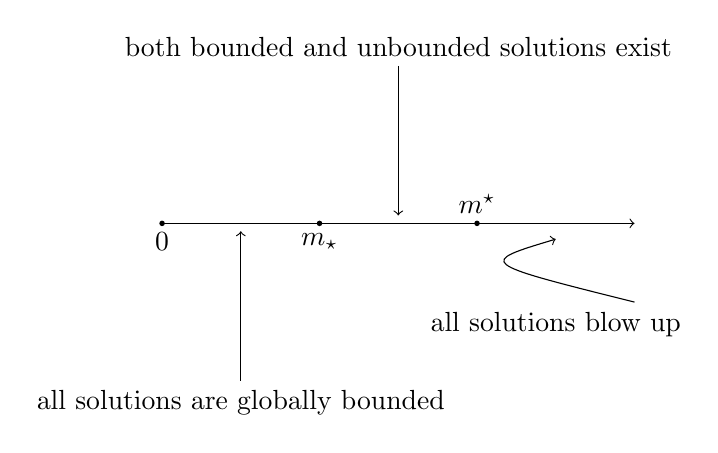
\begin{tikzpicture}
\coordinate (0) at (0,0); 
\coordinate (m) at (2,0);
\coordinate (M) at (4,0);
\coordinate (axis) at (6,0);
\coordinate (b) at (1,-2);
\coordinate (bu) at (3,2);
\coordinate (u) at (5, -1);
\fill (0) circle (1pt);
\fill (m) circle (1pt);
\fill (M) circle (1pt);
%\fill (0) circle (1pt);
\node at (0) [below]{0};
\node at (m) [below]{$m_\star$};
\node at (M) [above]{$m^\star$};
\draw[->] (0,0)--(6,0);
\draw[->] (1,-2)..controls(1,-1.5)..(1,-0.1);
\node at (b) [below]{all solutions are globally bounded};
\draw[->] (3,2)..controls(3,1.5) and (3,0.5)..(3,0.1);
\node at (bu) [above]{both bounded and unbounded solutions exist};
\draw[->] (6,-1)..controls(4,-0.5) ..(5,-0.2);
\node at (u) [below]{all solutions blow up};
\end{tikzpicture}

\end{document}